% Oral-presentation slides for the Master's project.
% Built from the report (sections/*.tex) — final seeded results.
% Narrative order: problem -> idea (language-conditioned recovery) -> environment
% -> decomposition -> orchestrator -> datasets -> fine-tuning variants -> results.
% Keyword-style bullets: the presenter develops them orally.
% Build: export PATH="/home/students/texlive/2026/bin/x86_64-linux:$PATH"
%        latexmk -pdf -interaction=nonstopmode -halt-on-error slides.tex
\documentclass[aspectratio=169,10pt]{beamer}

\usepackage[T1]{fontenc}
\usepackage[utf8]{inputenc}
\usepackage{lmodern}
\usepackage{graphicx}
\usepackage{booktabs}
\usepackage{siunitx}
\usepackage{xcolor}
\usepackage{tikz}
\usetikzlibrary{arrows.meta,positioning,fit,backgrounds,calc}

\graphicspath{{../figures/}}

% ---------- clean built-in look (no external theme needed) ----------
\usetheme{default}
\useinnertheme{circles}
\setbeamertemplate{navigation symbols}{}

\definecolor{epflred}{HTML}{B51F1F}
\definecolor{ink}{HTML}{222222}
\definecolor{accent}{HTML}{2C6E9B}
\definecolor{good}{HTML}{1B7F3B}

\setbeamercolor{structure}{fg=epflred}
\setbeamercolor{title}{fg=epflred}
\setbeamercolor{frametitle}{fg=white,bg=epflred}
\setbeamercolor{itemize item}{fg=epflred}
\setbeamercolor{itemize subitem}{fg=accent}
\setbeamercolor{block title}{fg=white,bg=accent}
\setbeamercolor{block body}{bg=accent!8}
\setbeamerfont{frametitle}{series=\bfseries}
\setbeamerfont{title}{series=\bfseries}
\setbeamertemplate{frametitle}{%
  \nointerlineskip
  \begin{beamercolorbox}[wd=\paperwidth,ht=3.2ex,dp=1.2ex,leftskip=0.6em,rightskip=0.6em]{frametitle}%
    \usebeamerfont{frametitle}\insertframetitle%
  \end{beamercolorbox}%
}
\setbeamertemplate{footline}{%
  \leavevmode%
  \hbox{%
    \begin{beamercolorbox}[wd=.34\paperwidth,ht=2.4ex,dp=1ex,leftskip=.6em]{}%
      \color{gray}\footnotesize Gal Pascual%
    \end{beamercolorbox}%
    \begin{beamercolorbox}[wd=.5\paperwidth,ht=2.4ex,dp=1ex,center]{}%
      \color{gray}\footnotesize Enabling Recovery in VLA-Based Manipulation%
    \end{beamercolorbox}%
    \begin{beamercolorbox}[wd=.16\paperwidth,ht=2.4ex,dp=1ex,rightskip=.6em]{}%
      \hfill\color{gray}\footnotesize\insertframenumber\,/\,\inserttotalframenumber%
    \end{beamercolorbox}%
  }%
}
\setbeamertemplate{caption}{\raggedright\insertcaption\par}
\setlength{\parskip}{4pt}

\newcommand{\hl}[1]{\textcolor{epflred}{\textbf{#1}}}
\newcommand{\gn}[1]{\textcolor{good}{\textbf{#1}}}

% ---------- title metadata ----------
\title{Enabling Recovery in VLA-Based Robotic Manipulation}
\subtitle{Master's Project}
\author{Gal Pascual}
\institute{EPFL \,\textbullet\, CREATE Lab (Prof.\ Josie Hughes) \,\textbullet\, Sycamore Lab\\
\footnotesize Supervisors: A.\ Schlaginhaufen, C.\ Pan, T.\ Ni}
\date{June 2026}

\begin{document}

% ===== 1. Title =====
{\setbeamertemplate{footline}{}
\begin{frame}[plain]
  \centering
  
\includegraphics[height=1.6cm]{logo.png}\\[0.8em]
  {\usebeamerfont{title}\color{epflred}\LARGE Enabling Recovery in\\[2pt] VLA-Based Robotic Manipulation\par}
  \vspace{0.5em}
  {\large Master's Project}\\[1.2em]
  {\large\textbf{Gal Pascual}}\\[0.8em]
  EPFL \,\textbullet\, CREATE Lab (Prof.\ Josie Hughes) \,\textbullet\, Sycamore Lab\\[0.3em]
  {\footnotesize Supervisors: Andreas Schlaginhaufen, Cheng Pan, Tingting Ni}\\[1.0em]
  {\footnotesize June 2026}
\end{frame}}

% ===== 2. Problem / goal =====
\begin{frame}{The problem}
  \begin{itemize}
    \item \hl{Imitation learning} --- mimic demonstrations
    \item Demos = \hl{successes only}
    \item One slip $\rightarrow$ \hl{out of distribution} $\rightarrow$ lost
    \item Long horizon $\rightarrow$ errors \hl{compound}
    \item No failure \hl{detection}, no \hl{interruption}
  \end{itemize}
  \vfill
  \begin{block}{Goal}
    \hl{Detect} failures \; $\cdot$ \; \hl{recover} \; $\cdot$ \; keep the task moving
  \end{block}
\end{frame}

% ===== 3. Idea =====
\begin{frame}{The idea: recovery through language}
  \begin{itemize}
    \item \hl{VLA} (vision--language--action) --- policy conditioned on a \hl{language instruction}
    \item Instruction = a \hl{run-time control knob}
    \item Task $\rightarrow$ \hl{simple language-instructed steps}
    \item Check each step $\rightarrow$ \hl{retry} \,/\, \hl{switch target} with a new instruction
  \end{itemize}
  \vfill
  \textbf{Built:} \hl{subtask dataset} \; $\cdot$ \; \hl{orchestrator} \; $\cdot$ \; \hl{autonomous data} probe
\end{frame}

% ===== 4. Environment & task =====
\begin{frame}{Environment \& task}
  \begin{columns}[c]
    \begin{column}{0.52\textwidth}
      \begin{itemize}
        \item \hl{SO-101} arm --- Isaac Sim
        \item \hl{3 oranges $\rightarrow$ plate} \; $\cdot$ \; score 0--3
        \item Policy: \hl{SmolVLA} --- 2 cameras $+$ joints, \hl{no object poses}
        \item Long horizon --- thousands of steps
      \end{itemize}
    \end{column}
    \begin{column}{0.48\textwidth}
      \centering
      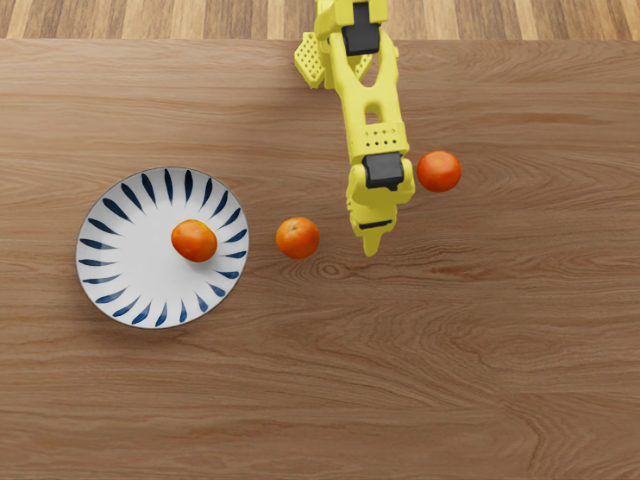
\includegraphics[width=\textwidth,height=0.42\textheight,keepaspectratio]{environment_top_view.png}\\[0.4em]
      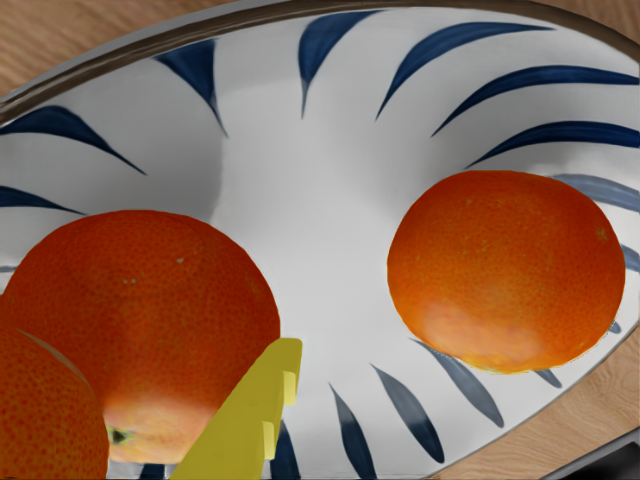
\includegraphics[width=0.72\textwidth,height=0.34\textheight,keepaspectratio]{environment_plate_closeup.png}\\
      {\footnotesize Top camera \,\textbullet\, wrist camera}
    \end{column}
  \end{columns}
\end{frame}

% ===== 5. Decomposition =====
\begin{frame}{Decomposing the task}
  \begin{itemize}
    \item \hl{GRASP $\rightarrow$ LIFT $\rightarrow$ PLACE} --- each a \hl{checkpoint}, outcome \hl{verified}
    \item GRASP targets \hl{by position} --- ``left / middle / right orange''
    \item LIFT gated on a \hl{secure grasp} --- centred $+$ contact force
    \item Comparison: \hl{monotask} --- one prompt, end-to-end
  \end{itemize}
  \vfill
  \begin{columns}[c]
    \column{0.32\textwidth}\centering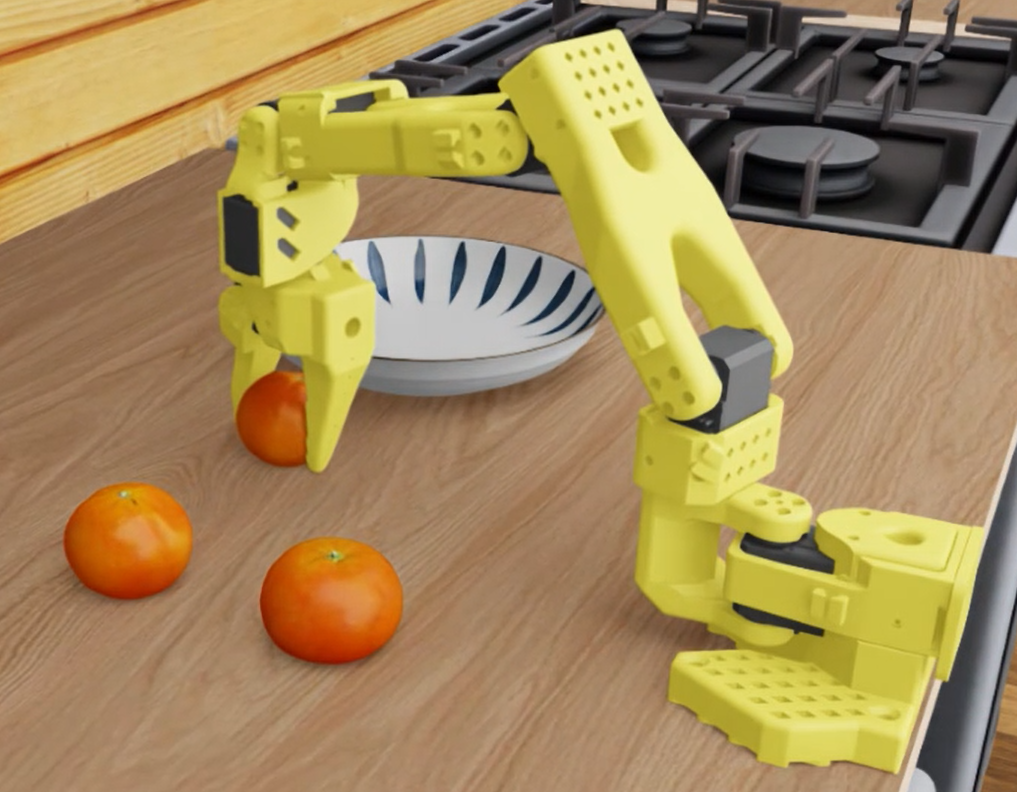
\includegraphics[height=2.4cm]{grasp.png}\\\textbf{GRASP}
    \column{0.32\textwidth}\centering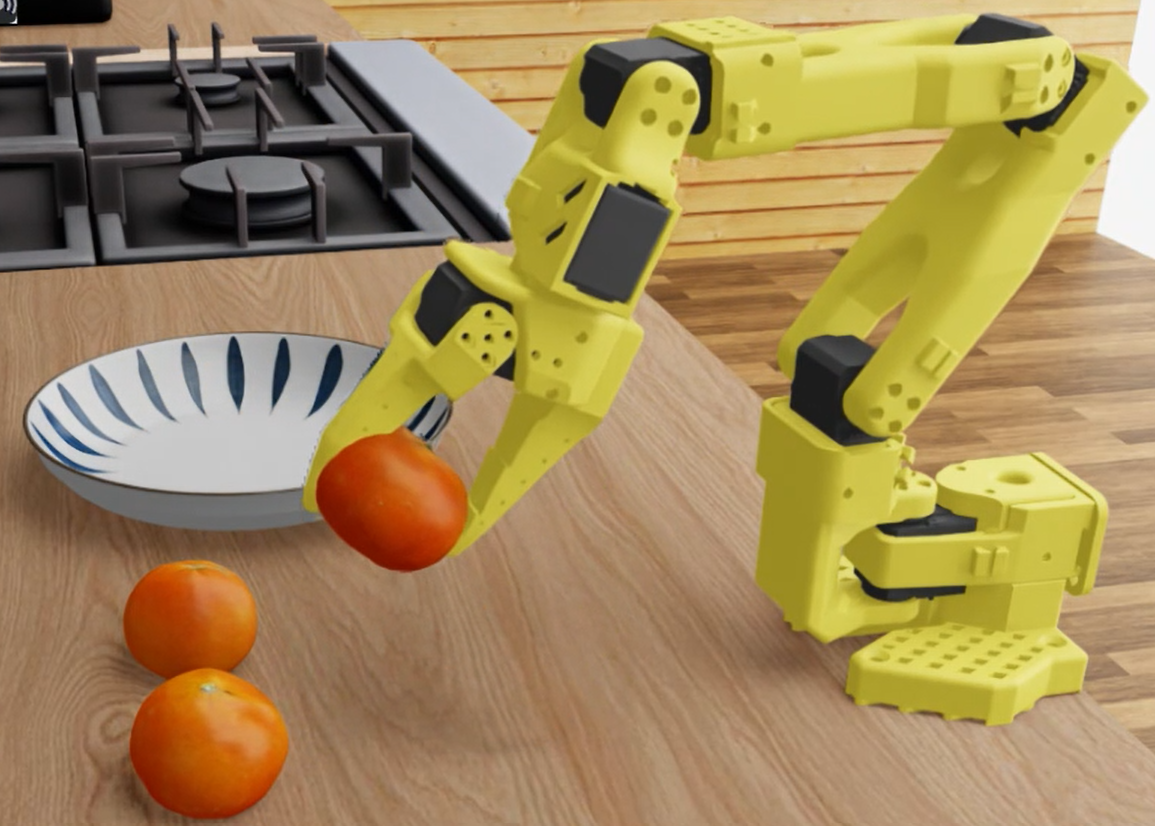
\includegraphics[height=2.4cm]{pick.png}\\\textbf{LIFT}
    \column{0.32\textwidth}\centering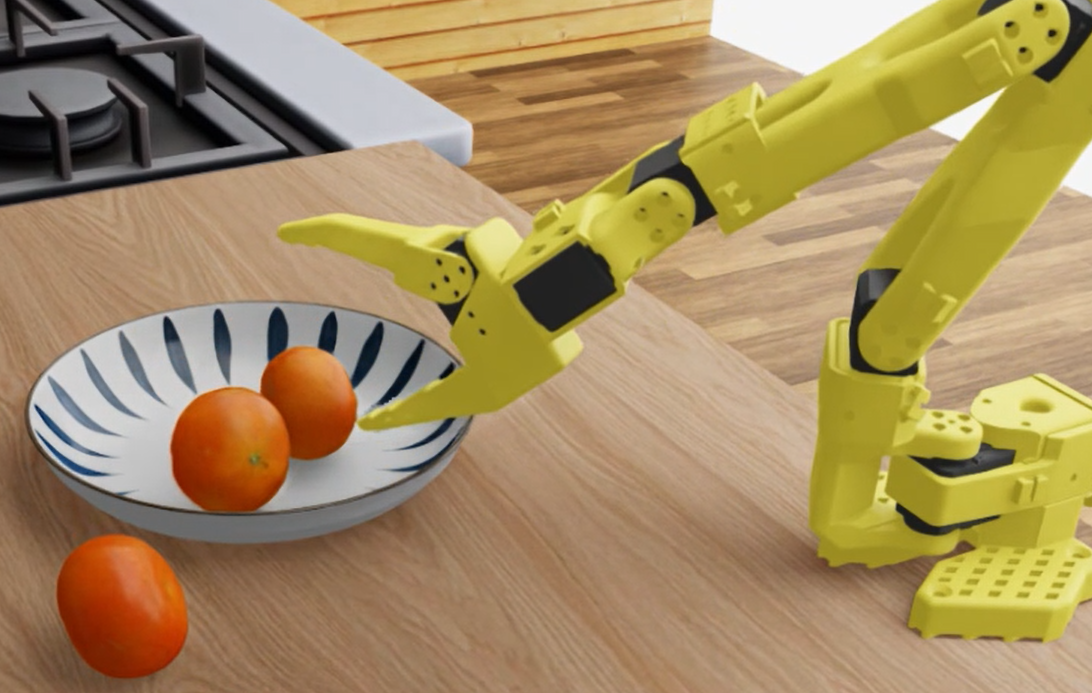
\includegraphics[height=2.4cm]{place.png}\\\textbf{PLACE}
  \end{columns}
\end{frame}

% ===== 6. Orchestrator + recovery =====
\begin{frame}{Orchestrator \& recovery}
  \begin{columns}[c]
    \begin{column}{0.54\textwidth}
      \begin{itemize}
        \item Checks: \hl{privileged sim state} --- policy never sees it
        \item \hl{Timeout} = step budget $\rightarrow$ detection trigger
        \item \hl{Level-1 retry} --- \textbf{same} orange
        \item \hl{Level-2 redirect} --- \textbf{different} orange, task keeps scoring
        \item \hl{Home reset} --- precondition; target switch only \hl{far from oranges}
      \end{itemize}
    \end{column}
    \begin{column}{0.46\textwidth}
      \centering
      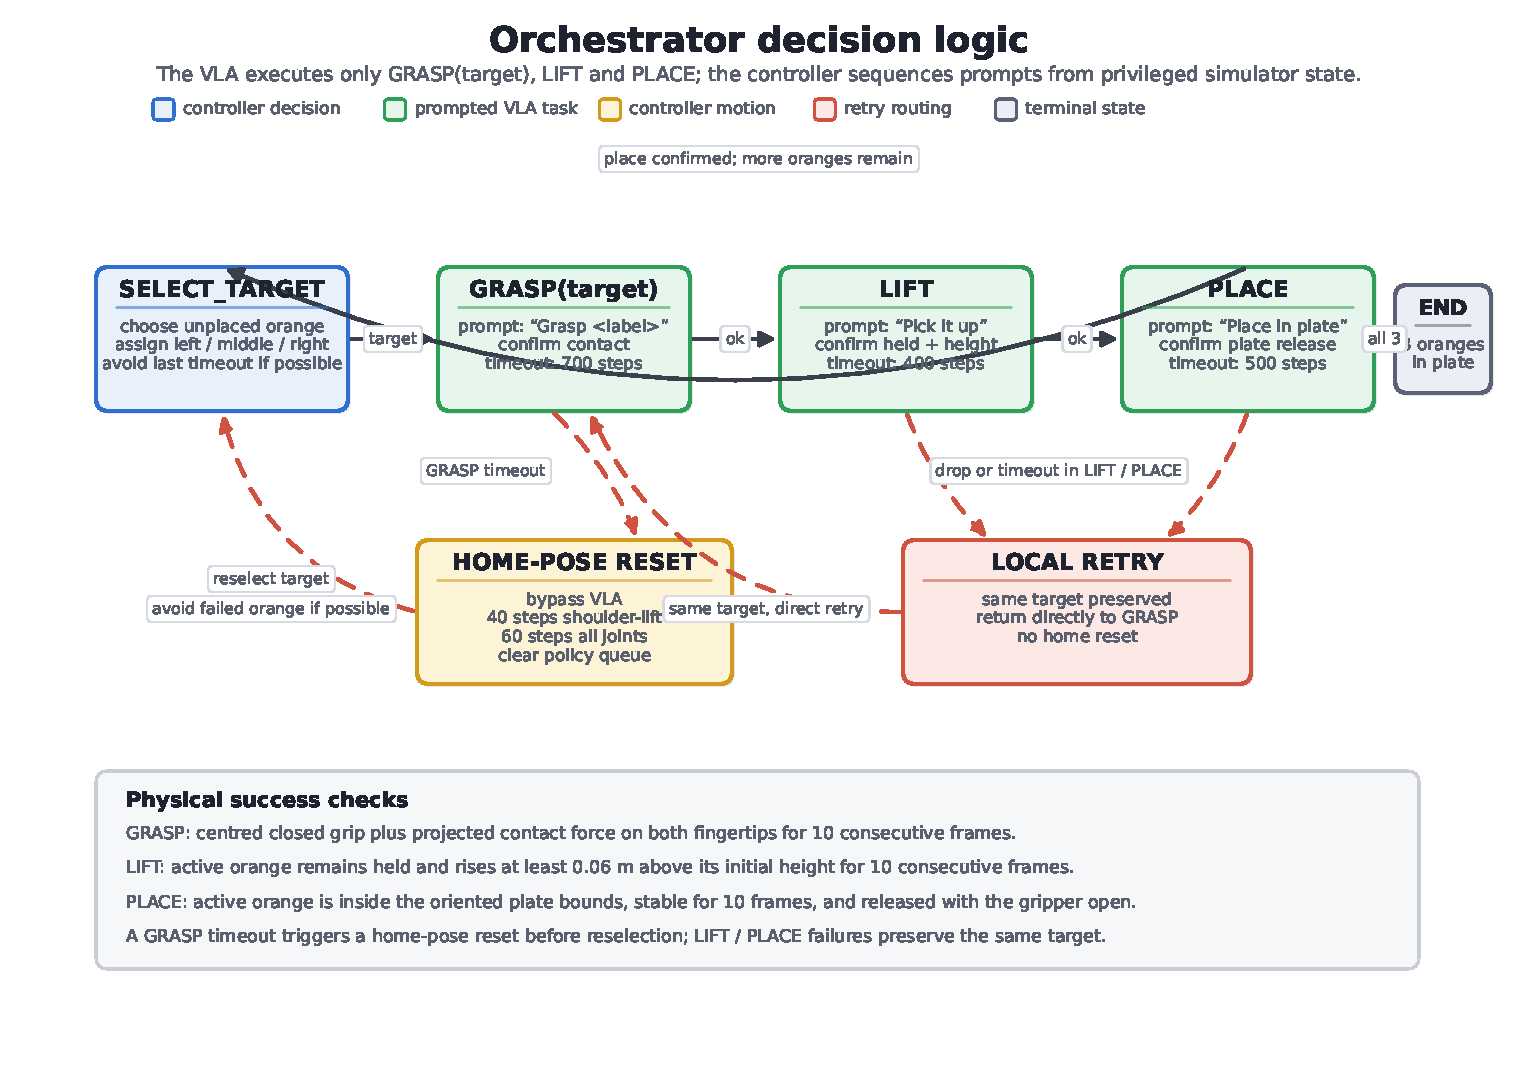
\includegraphics[width=\textwidth]{orchestrator_decision_flow.pdf}
    \end{column}
  \end{columns}
\end{frame}

% ===== 7. Datasets =====
\begin{frame}{Datasets}
  \begin{columns}[c]
    \begin{column}{0.52\textwidth}
      \begin{itemize}
        \item \hl{846 Teleop} subtask episodes --- gamepad \; $\cdot$ \; \hl{random pick order} \; $\cdot$ \; \hl{freeze tail}
        \item Flattened $\rightarrow$ \hl{monotask} set --- matched comparison
        \item \hl{$+414$ Auto} --- self-run, successes only $\rightarrow$ \hl{Teleop+Auto}
        \item Baseline: \hl{60 public} end-to-end demos
      \end{itemize}
    \end{column}
    \begin{column}{0.48\textwidth}
      \centering
      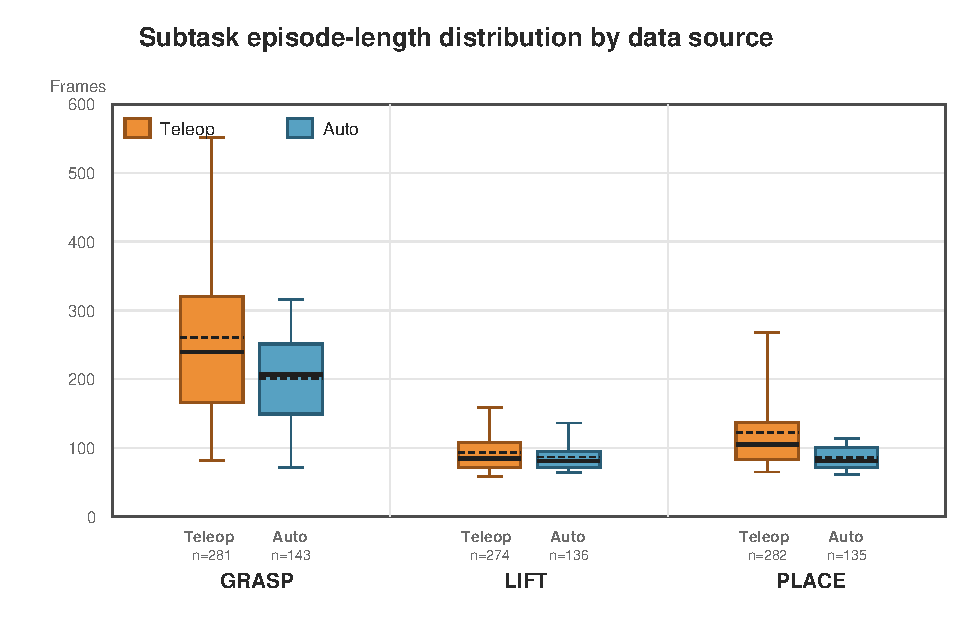
\includegraphics[width=\textwidth]{dataset_composition.pdf}
    \end{column}
  \end{columns}
\end{frame}

% ===== 8. Fine-tuning variants (schematic) =====
\begin{frame}{Fine-tuning: three variants}
  \centering
  \resizebox{0.92\textwidth}{!}{%
    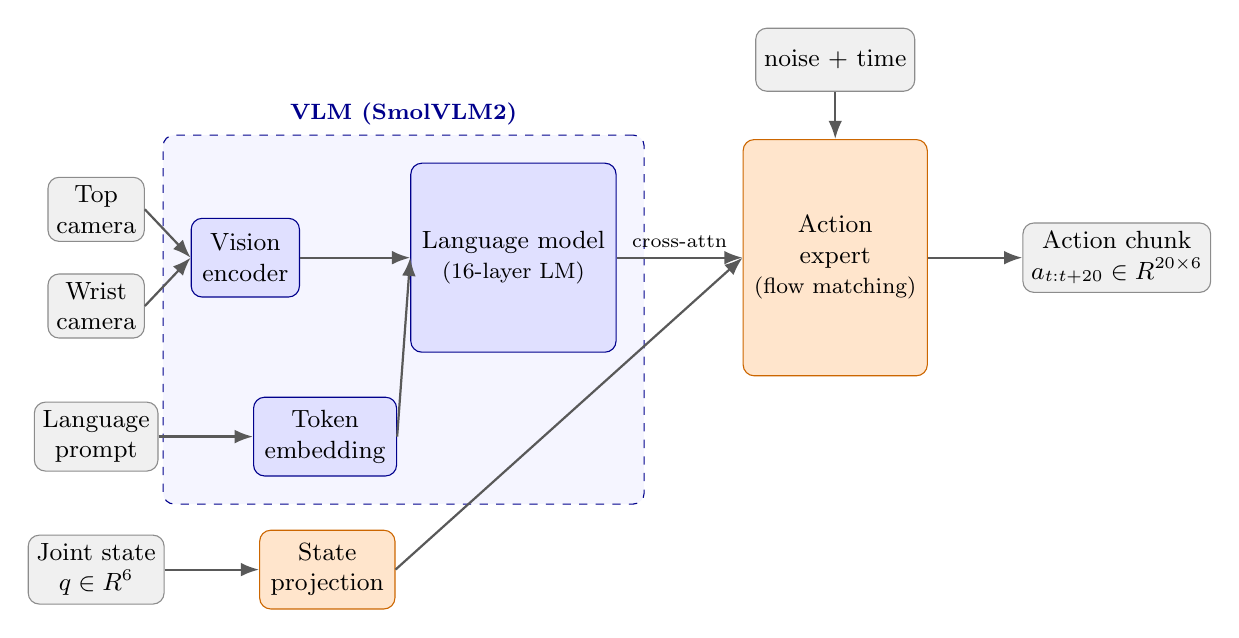
\begin{tikzpicture}[
        font=\small, >=Latex, node distance=6mm,
        frozen/.style={draw=blue!55!black, fill=blue!12, rounded corners, align=center, minimum height=10mm, inner sep=4pt},
        trained/.style={draw=orange!80!black, fill=orange!20, rounded corners, align=center, minimum height=10mm, inner sep=4pt},
        io/.style={draw=black!45, fill=black!6, rounded corners, align=center, minimum height=8mm, inner sep=3pt},
        arr/.style={->, thick, draw=black!65},
    ]
        \node[io] (front) {Top\\camera};
        \node[io, below=4mm of front] (wrist) {Wrist\\camera};
        \node[io, below=8mm of wrist] (prompt) {Language\\prompt};
        \node[io, below=8mm of prompt] (state) {Joint state\\$q\in\mathbb{R}^{6}$};
        \node[frozen, right=12mm of $(front)!0.5!(wrist)$] (venc) {Vision\\encoder};
        \node[frozen, right=12mm of prompt] (emb) {Token\\embedding};
        \node[trained, right=12mm of state] (sproj) {State\\projection};
        \node[frozen, right=14mm of venc, minimum height=24mm] (vlm) {Language model\\\footnotesize(16-layer LM)};
        \node[trained, right=16mm of vlm, minimum height=30mm] (expert) {Action\\expert\\\footnotesize(flow matching)};
        \node[io, right=12mm of expert] (act) {Action chunk\\$a_{t:t+20}\in\mathbb{R}^{20\times 6}$};
        \node[io, above=6mm of expert] (noise) {noise $+$ time};
        \begin{scope}[on background layer]
            \node[draw=blue!55!black, dashed, rounded corners, fill=blue!4, inner sep=3.5mm,
                  fit=(venc)(emb)(vlm),
                  label={[blue!55!black, font=\footnotesize\bfseries]above:VLM (SmolVLM2)}] (vlmbox) {};
        \end{scope}
        \draw[arr] (front.east) -- (venc.west);
        \draw[arr] (wrist.east) -- (venc.west);
        \draw[arr] (prompt.east) -- (emb.west);
        \draw[arr] (state.east) -- (sproj.west);
        \draw[arr] (venc.east) -- (vlm.west);
        \draw[arr] (emb.east) -- (vlm.west);
        \draw[arr] (vlm.east) -- node[above, font=\scriptsize]{cross-attn} (expert.west);
        \draw[arr] (sproj.east) -- (expert.west);
        \draw[arr] (noise.south) -- (expert.north);
        \draw[arr] (expert.east) -- (act.west);
    \end{tikzpicture}}

  \vspace{0.5em}
  {\footnotesize\hl{Standard} action expert only ($\sim$100M) \; $\cdot$ \; \hl{Partial} $+$ language model ($\sim$316M) \; $\cdot$ \; \hl{Full} $+$ vision (450M)}
\end{frame}

% ===== 9. Results: outcomes, all models =====
\begin{frame}{Results: outcomes across all models}
  \begin{columns}[c]
    \begin{column}{0.40\textwidth}
      \begin{itemize}
        \item \hl{100 seeded} episodes / model
        \item \gn{$\geq$1 orange: 97\%} vs.\ 56\% --- rarely empty-handed
        \item Full completions: \hl{no reliable gain} (standard)
        \item \hl{Full tuning}: \emph{every} family $\uparrow$ --- best \gn{61\%}
      \end{itemize}
    \end{column}
    \begin{column}{0.60\textwidth}
      \centering
      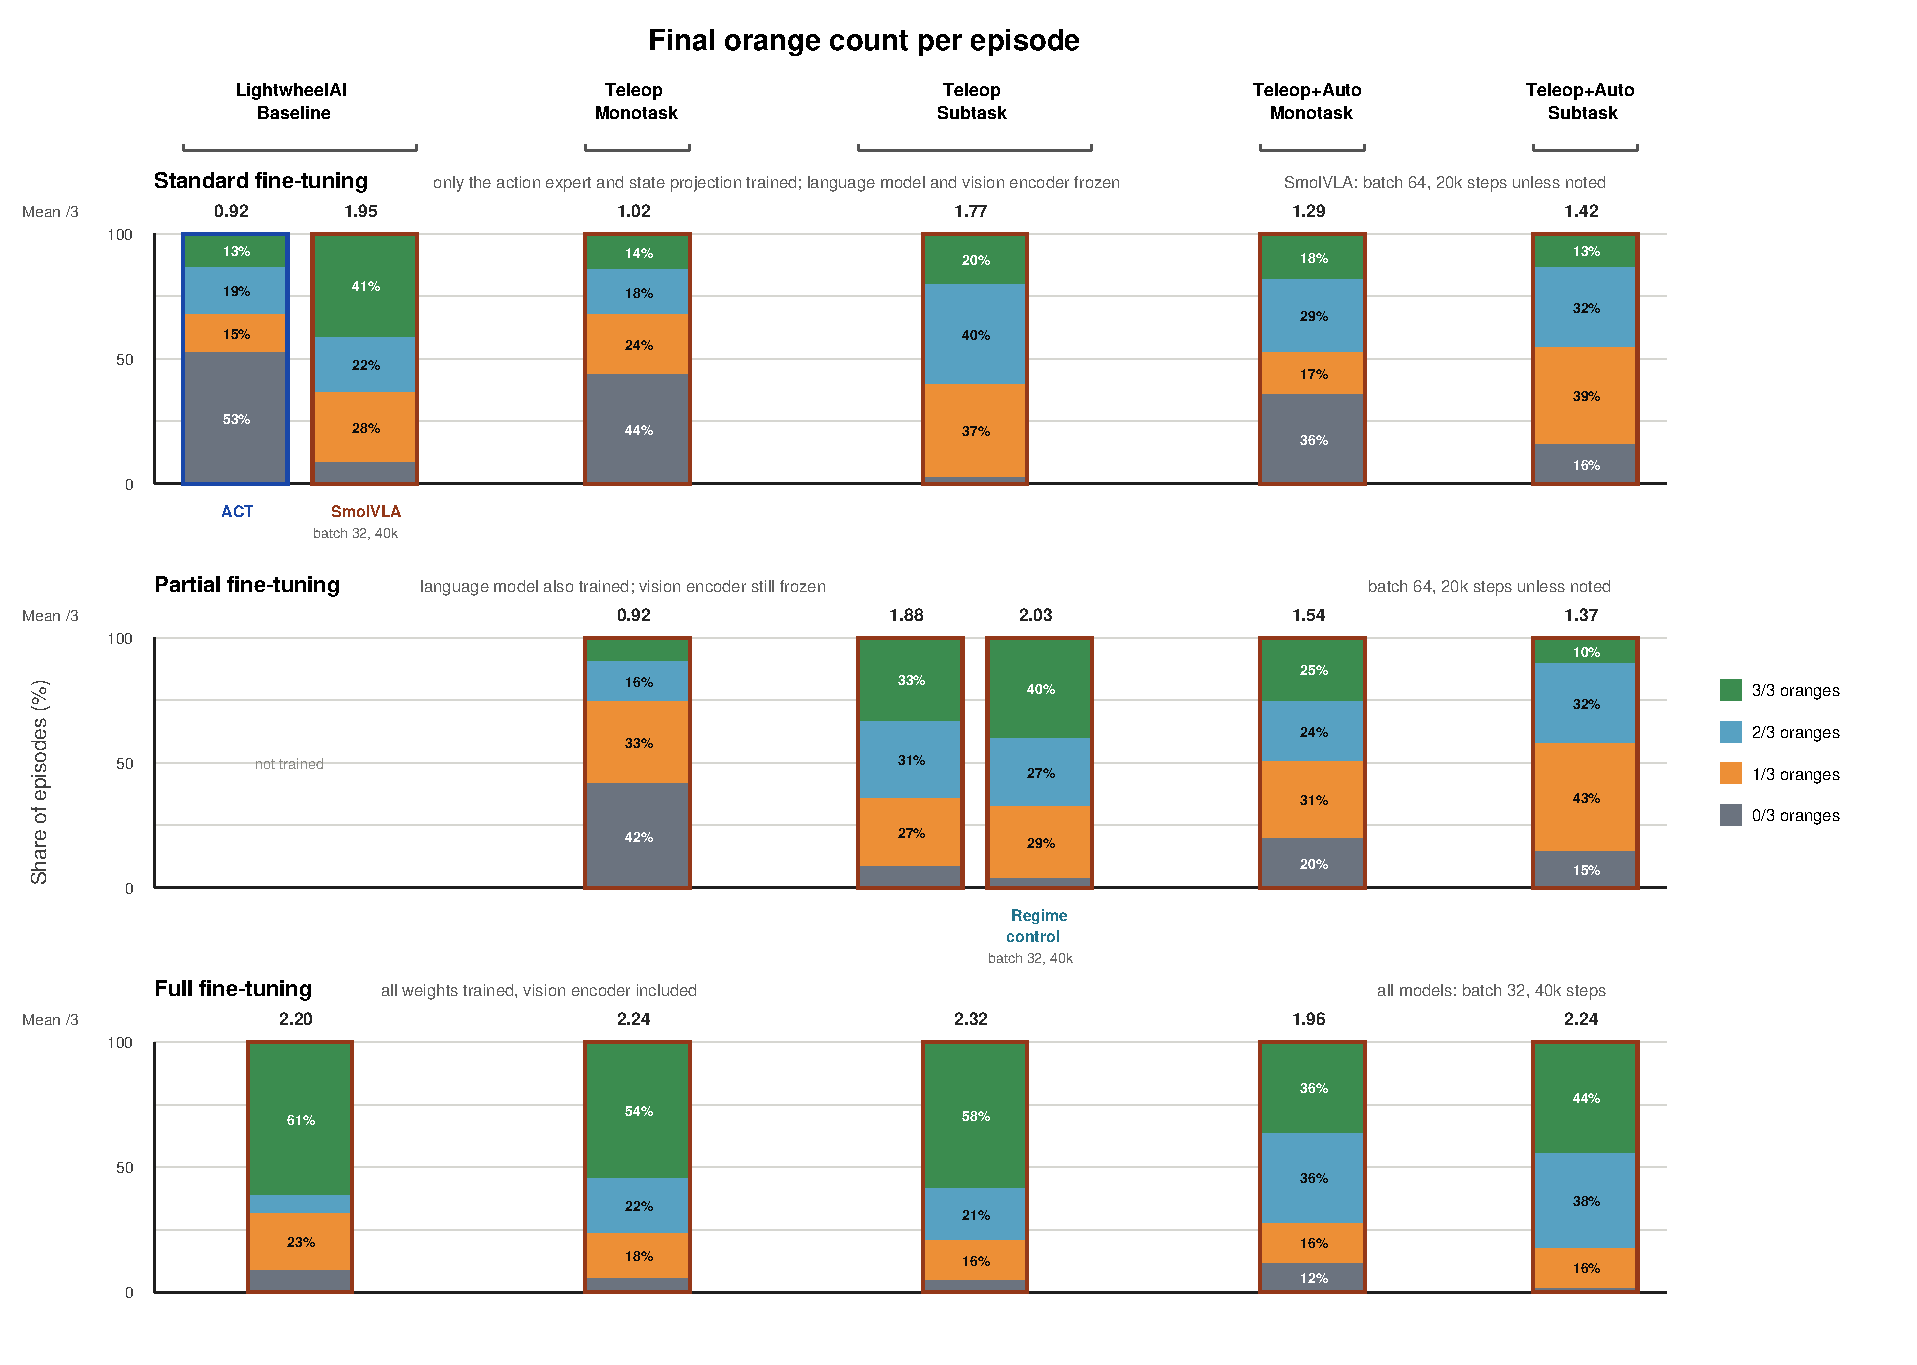
\includegraphics[width=\linewidth,height=0.84\textheight,keepaspectratio]{orange_outcome_recipes.pdf}
    \end{column}
  \end{columns}
\end{frame}

% ===== 10. Results: grasp bottleneck =====
\begin{frame}{Grasp acquisition is the bottleneck}
  \begin{itemize}
    \item GRASP: \hl{$\sim$37\%} $\rightarrow$ \gn{55\%} (full tuning)
    \item LIFT / PLACE: \hl{already reliable}
    \item Monotask lift (no gate): \hl{56\% $\rightarrow$ 94\%}
  \end{itemize}
  \vfill
  \centering
  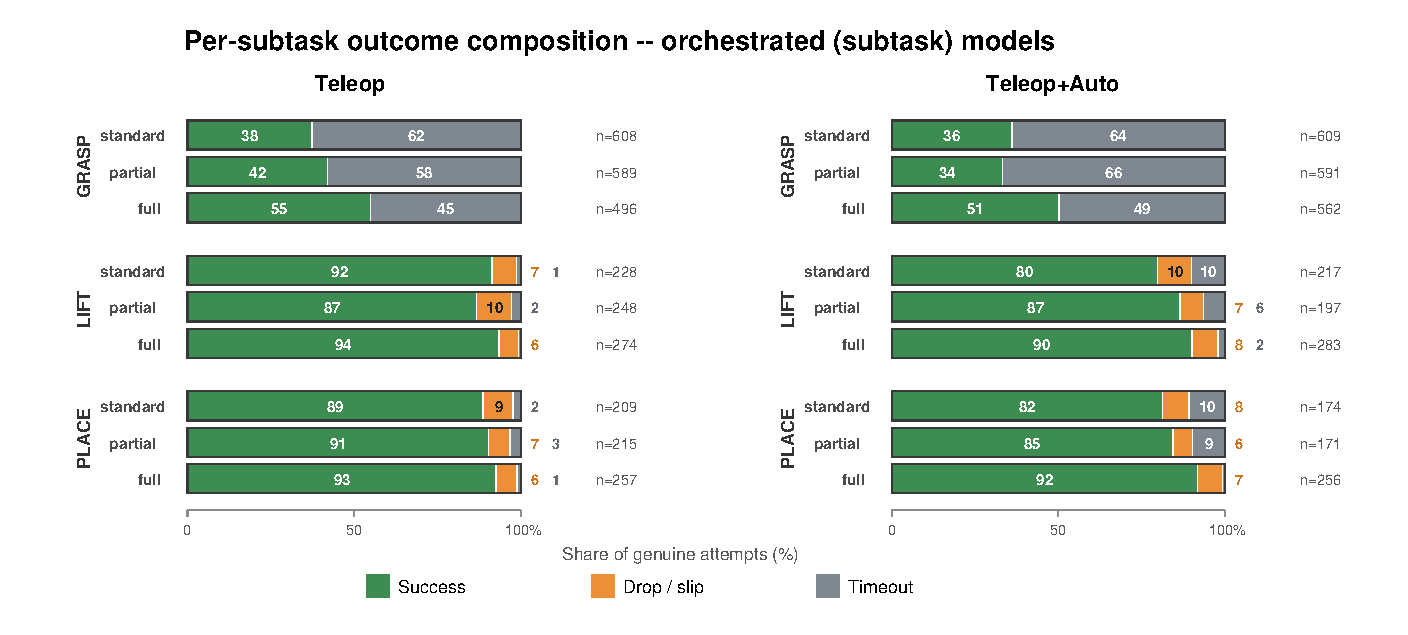
\includegraphics[width=\textwidth,height=0.62\textheight,keepaspectratio]{failure_modes_variants_subtask.pdf}
\end{frame}

% ===== 11. Results: recovery at matched stalls =====
\begin{frame}{Recovery, compared at matched stalls}
  {\footnotesize \hl{Stall} = one grasp budget stuck on one orange (monotask intent $\approx$ \emph{proximity}). What happens next?}
  \vfill
  \centering\small
  \begin{tabular}{llccc}
    \toprule
    Training & Form. & Redirected & Placed after & \dots via \emph{different} orange \\
    \midrule
    Teleop      & Monotask          & 53.5\%     & 31.4\%        & 16.3\% \\
    Teleop      & \textbf{Subtask}  & \gn{100\%} & \gn{71.2\%}   & \gn{53.4\%} \\
    \midrule
    Teleop+Auto & Monotask          & 45.2\%     & 34.4\%        & 17.2\% \\
    Teleop+Auto & \textbf{Subtask}  & \gn{100\%} & \gn{43.2\%}   & \gn{33.7\%} \\
    \bottomrule
  \end{tabular}
  \vfill
  \begin{itemize}
    \item Orchestrator: \hl{redirects every time} \; $\cdot$ \; monotask: \hl{$\sim$half}
    \item Gap $=$ \hl{different-orange column} \; $\cdot$ \; Level-1 marginal
  \end{itemize}
\end{frame}

% ===== 12. Results: obedience =====
\begin{frame}{Does it grasp the orange it was told to?}
  \begin{columns}[c]
    \begin{column}{0.42\textwidth}
      \begin{itemize}
        \item Obeys \hl{64--73\%}
        \item \hl{More VLM $\neq$ better} --- partial 67\%, full 64\%
        \item Misses \hl{leftward} --- \emph{right} worst (27--47\%)
      \end{itemize}
    \end{column}
    \begin{column}{0.58\textwidth}
      \centering
      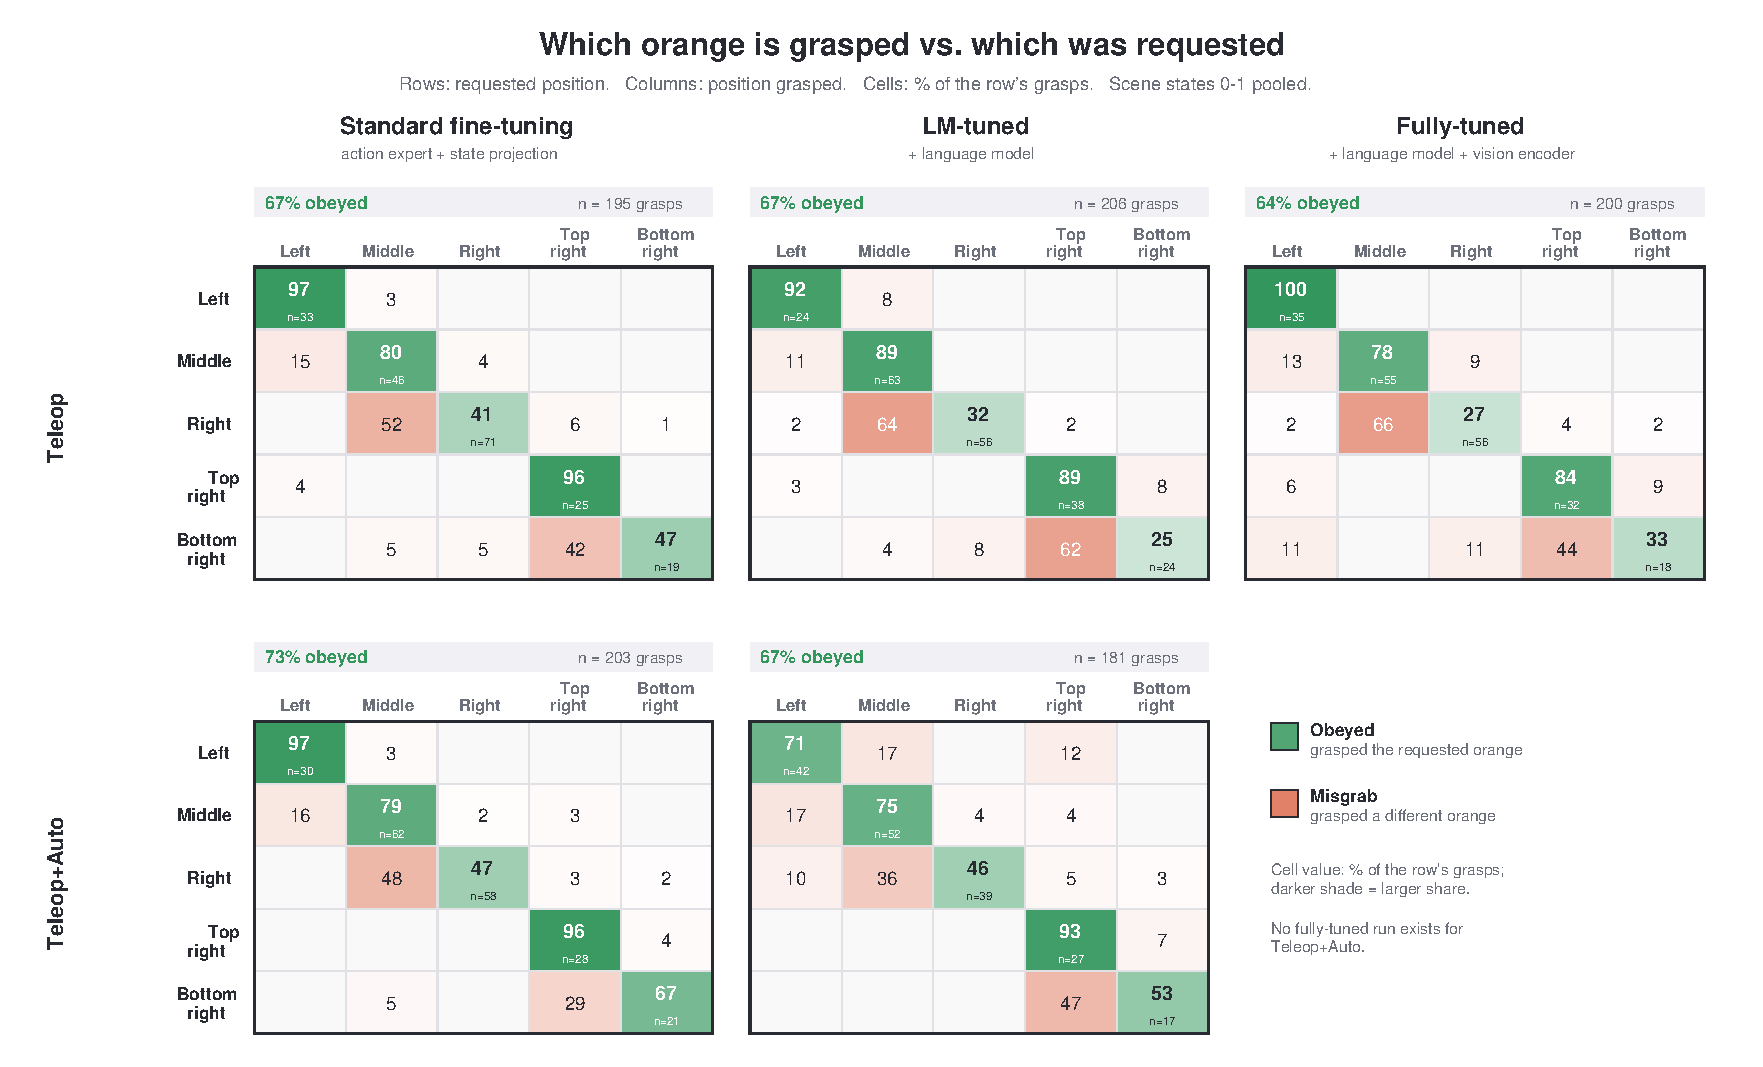
\includegraphics[width=\linewidth,height=0.84\textheight,keepaspectratio]{grasp_obedience_confusion.pdf}
    \end{column}
  \end{columns}
\end{frame}

% ===== 13. Takeaways + future =====
\begin{frame}{Takeaways \& future work}
  \begin{itemize}
    \item Helps \hl{most where grasping is weak} --- rarely empty-handed (Level-2)
    \item \hl{Cannot fix a weak grasp} --- a \hl{stronger policy} did (vision), not more structure
    \item Two \hl{complementary levers} --- better grasping $+$ graceful failure
    \item This task: the orchestration's \hl{floor}, not its ceiling
  \end{itemize}
  \vfill
  \textbf{Next:} RL / targeted grasp demos \; $\cdot$ \; \hl{from-any-state} data \; $\cdot$ \; \hl{VLM success monitor}
\end{frame}

% ===== 14. Thanks =====
{\setbeamertemplate{footline}{}
\begin{frame}[plain]
  \centering
  \vspace{1.2cm}
  {\color{epflred}\Huge\textbf{Thank you}}\\[0.8em]
  {\large Questions?}\\[1.4em]
  {\footnotesize Gal Pascual \,\textbullet\, EPFL CREATE Lab / Sycamore Lab}
\end{frame}}

% =========================================================
% ===============   BACKUP  (for Q&A)   ===================
% =========================================================
{\setbeamercolor{frametitle}{fg=white,bg=ink}

% ----- B1: monotask failure composition -----
\begin{frame}{Backup: monotask lift/place composition}
  \centering
  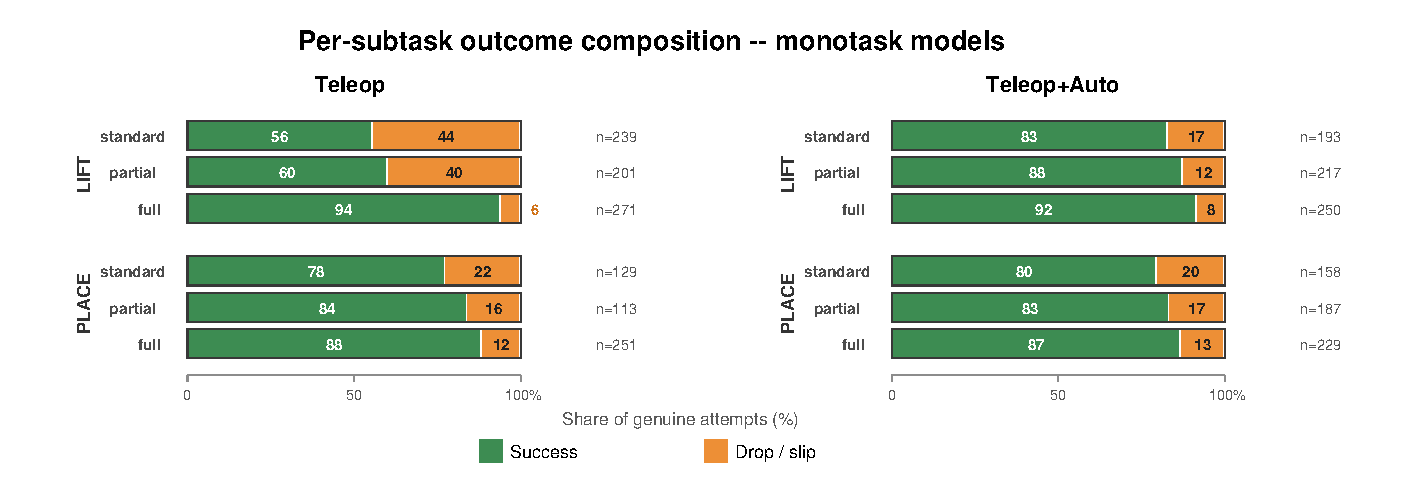
\includegraphics[width=\textwidth,height=0.62\textheight,keepaspectratio]{failure_modes_variants_monotask.pdf}\\
  {\footnotesize Full fine-tuning sharply cuts lift failures --- Teleop \hl{56\% $\rightarrow$ 94\%} success.}
\end{frame}

% ----- B2: baseline ACT vs SmolVLA -----
\begin{frame}{Backup: baseline --- is it the policy class?}
  \begin{columns}[c]
    \begin{column}{0.54\textwidth}
      \begin{itemize}
        \item 60 public end-to-end demos, one fixed prompt (\hl{monotask})
        \item \hl{SmolVLA $>$ ACT} --- 43\% vs.\ 13\%; still only \hl{43 / 100}
        \item[$\Rightarrow$] Limit $=$ \hl{execution structure}, not policy expressiveness
      \end{itemize}
    \end{column}
    \begin{column}{0.46\textwidth}
      \centering
      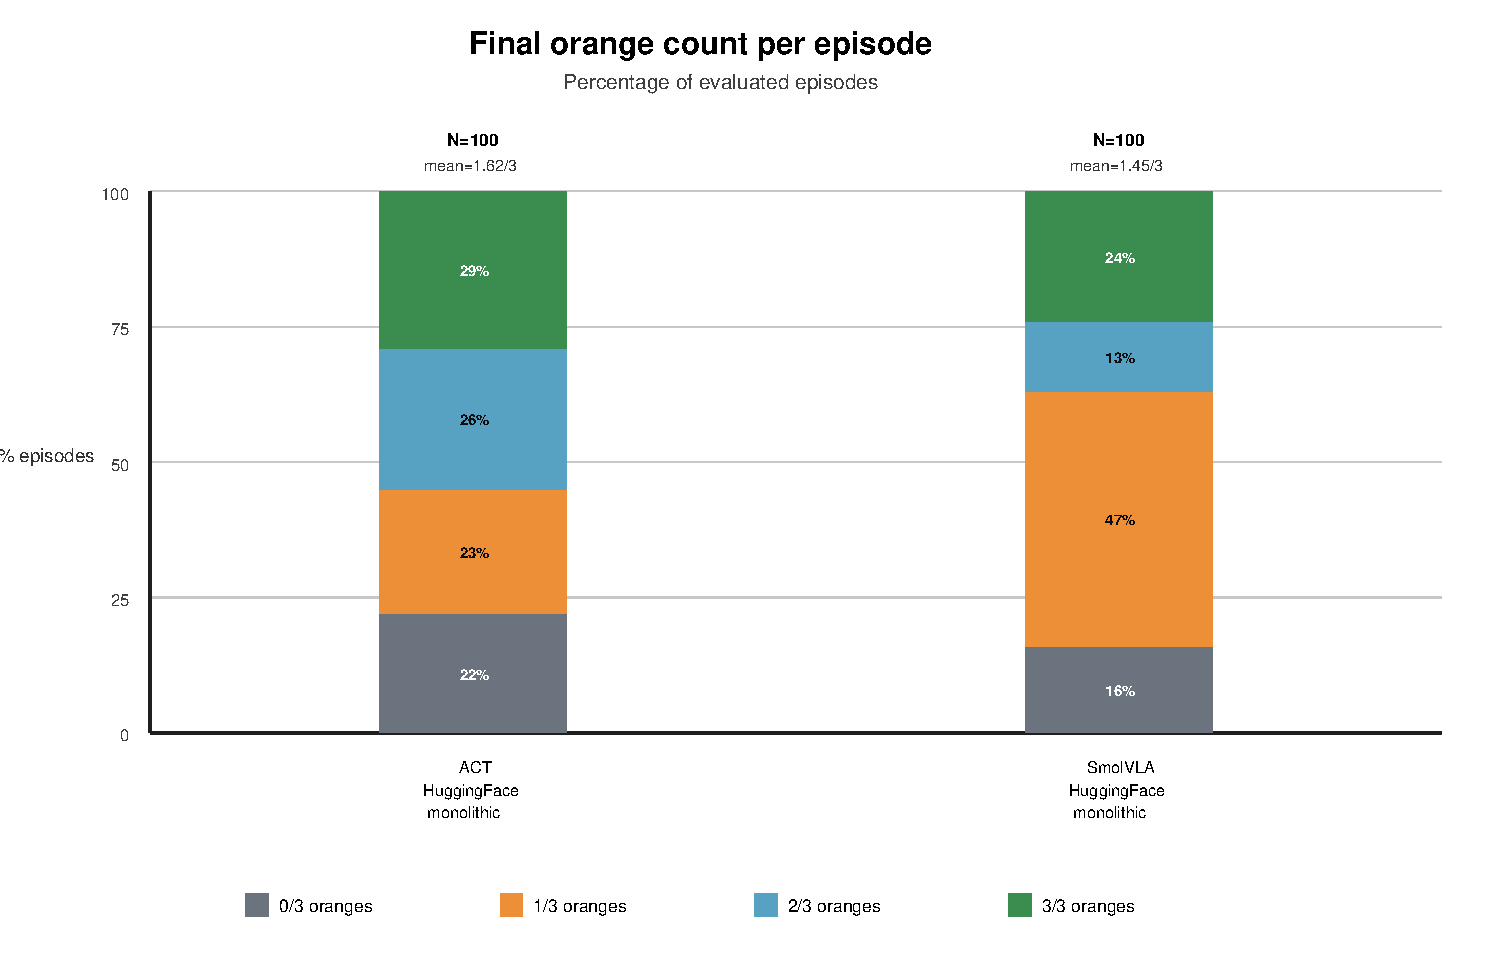
\includegraphics[width=\textwidth]{baseline_comparison.pdf}
    \end{column}
  \end{columns}
\end{frame}

% ----- B3: limitations -----
\begin{frame}{Backup: limitations}
  \begin{itemize}
    \item \hl{Privileged supervision} --- deployment needs perception
    \item \hl{Matched-regime confound} --- full variant: batch 32 / 40k (controls bound it)
    \item \hl{Composite-label inconsistency} --- labels by eye vs.\ 3\,cm rule
    \item \hl{Limited sampling} --- 100 episodes / model
    \item \hl{Slow execution} --- slow teleop $\rightarrow$ long rollouts
  \end{itemize}
\end{frame}

}

\end{document}
